\documentclass[11pt]{article}
\usepackage[margin=1in]{geometry}
\usepackage[T1]{fontenc}
\usepackage[utf8]{inputenc}
\usepackage{lmodern}
\usepackage{microtype}
\usepackage{amsmath}
\usepackage{booktabs}
\usepackage{multirow}
\usepackage{graphicx}
\usepackage{xcolor}
\usepackage{listings}
\usepackage{tikz}
\usetikzlibrary{positioning,arrows.meta,fit,backgrounds,calc}
\usepackage[numbers,sort&compress]{natbib}
\usepackage[colorlinks=true,linkcolor=blue!60!black,citecolor=blue!60!black,urlcolor=blue!60!black]{hyperref}

\graphicspath{{figures/}}
\lstset{basicstyle=\ttfamily\small,breaklines=true,columns=fullflexible,frame=single,framerule=0.3pt}
\newcommand{\pmstd}[2]{#1{\scriptsize$\,\pm\,$#2}}

\title{\textbf{TinySQL: A 125M-Parameter Text-to-SQL Model\\Built and Pretrained From Scratch on 4.5B Tokens}}
\author{Aditya Narayan Jha\\AI Engineer\\\url{https://github.com/aditya0929/tinysql}}
\date{October 2026}

\begin{document}
\maketitle

\begin{abstract}
We describe TinySQL-125M, a decoder-only language model for text-to-SQL in which every component of the model path is written from scratch: a byte-level BPE tokenizer, the transformer itself (grouped-query attention, rotary embeddings, SwiGLU, RMSNorm), the optimizer, the training loop, the data pipeline, a grammar-constrained decoder and the evaluation harness. The model is pretrained for about 46 hours on a single NVIDIA L4 GPU on 4.5B tokens of educational web text and SQL code, then fine-tuned on WikiSQL. To make the result interpretable, we fine-tune four public models of similar size (GPT-2 124M, Pythia-160M, SmolLM2-135M and SmolLM2-360M) with an identical recipe, sweep the learning rate for every model, average over three seeds, train our architecture without pretraining as a control, and report confidence intervals and paired significance tests throughout. On the WikiSQL test set, TinySQL reaches 77.95\,$\pm$\,0.18\% execution accuracy with greedy decoding and 80.39\,$\pm$\,0.20\% with schema- and value-constrained decoding (official evaluator: 78.03\% and 80.50\%). This is about one point below GPT-2 and 17 points above Pythia-160M, which was pretrained on 67$\times$ more tokens; SmolLM2-135M, pretrained on 2T tokens (about 440$\times$ more), is 4.6 points ahead. Pretraining accounts for 41 points of accuracy. Constrained decoding never turned one of our model's correct answers into a wrong one in any paired comparison we ran. Small-scale ablations show that rotary embeddings and tied embeddings matter far more than grouped-query attention or an SQL-heavy pretraining mix, and a hand audit suggests that most remaining aggregation errors are label errors in WikiSQL. All code, results and the 166 tests that verify the components are public.
\end{abstract}

\section{Introduction}

Small language models are attractive for text-to-SQL: they run on a CPU, can be deployed next to a database, and are cheap to fine-tune. Most small models available today are pretrained by well-resourced teams on trillions of tokens. This report asks a narrower question: \emph{how far can a single person get on a standard text-to-SQL benchmark with a model whose every part they built themselves, on a pretraining budget of a few billion tokens and one rented GPU?}

To answer it credibly, the system is built without any pretrained weights, pretrained tokenizers or high-level modeling libraries (Section~\ref{sec:system}), and the evaluation is designed so that differences can be attributed (Section~\ref{sec:setup}): every baseline gets the same fine-tuning recipe and its own learning-rate sweep, main results are averaged over seeds, the test set is used once, and comparisons are paired and tested for significance.

\paragraph{Contributions.}
\begin{itemize}
  \item A complete, tested, from-scratch text-to-SQL stack: tokenizer, Llama-style model~\cite{touvron2023llama}, optimizer, a data pipeline with deduplication and benchmark decontamination, a grammar-constrained decoder, and evaluation code (Section~\ref{sec:system}).
  \item A controlled comparison on WikiSQL~\cite{zhong2017seq2sql} against four public models of similar size, with learning-rate sweeps, three seeds, a no-pretraining control, bootstrap confidence intervals and McNemar tests (Section~\ref{sec:results}).
  \item Evidence that a 4.5B-token model trained on a deliberate web+SQL mix comes within about one point of GPT-2 and well above Pythia-160M at this task, and that constrained decoding helps weaker models more without ever hurting ours.
  \item Ablations of four design choices (Section~\ref{sec:ablations}), a failure analysis, and a hand audit of aggregation labels (Section~\ref{sec:failures}).
\end{itemize}

\begin{figure}[!htbp]
\centering
\resizebox{\linewidth}{!}{% End-to-end pipeline: data -> tokenizer -> pretraining -> fine-tuning -> decoding -> evaluation.
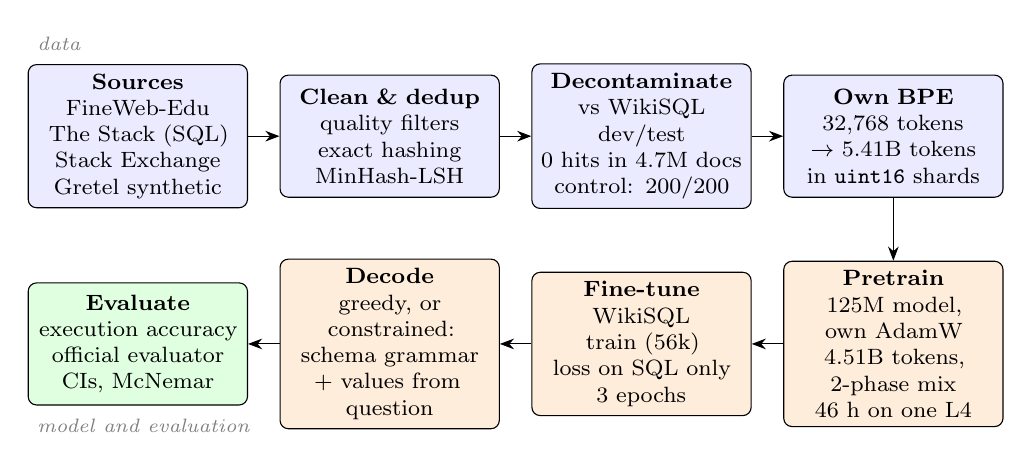
\begin{tikzpicture}[
  font=\footnotesize,
  >={Stealth[length=1.8mm]},
  stage/.style={draw, rounded corners=3pt, align=center, minimum height=1.55cm, text width=2.55cm, fill=#1},
  stage/.default=white,
  node distance=4mm,
]
\node[stage=blue!8] (src) {\textbf{Sources}\\FineWeb-Edu\\The Stack (SQL)\\Stack Exchange\\Gretel synthetic};
\node[stage=blue!8, right=of src] (clean) {\textbf{Clean \& dedup}\\quality filters\\exact hashing\\MinHash-LSH};
\node[stage=blue!8, right=of clean] (decon) {\textbf{Decontaminate}\\vs WikiSQL dev/test\\0 hits in 4.7M docs\\control: 200/200};
\node[stage=blue!8, right=of decon] (tok) {\textbf{Own BPE}\\32,768 tokens\\$\rightarrow$ 5.41B tokens\\in \texttt{uint16} shards};

\node[stage=orange!14, below=8mm of tok] (pre) {\textbf{Pretrain}\\125M model, own AdamW\\4.51B tokens, 2-phase mix\\46 h on one L4};
\node[stage=orange!14, left=of pre] (ft) {\textbf{Fine-tune}\\WikiSQL train (56k)\\loss on SQL only\\3 epochs};
\node[stage=orange!14, left=of ft] (dec) {\textbf{Decode}\\greedy, or constrained:\\schema grammar\\+ values from question};
\node[stage=green!12, left=of dec] (eval) {\textbf{Evaluate}\\execution accuracy\\official evaluator\\CIs, McNemar};

\draw[->] (src) -- (clean);
\draw[->] (clean) -- (decon);
\draw[->] (decon) -- (tok);
\draw[->] (tok) -- (pre);
\draw[->] (pre) -- (ft);
\draw[->] (ft) -- (dec);
\draw[->] (dec) -- (eval);

\node[anchor=south west, font=\scriptsize\itshape, gray] at ($(src.north west)+(0,0.05)$) {data};
\node[anchor=north west, font=\scriptsize\itshape, gray] at ($(eval.south west)+(0,-0.05)$) {model and evaluation};
\end{tikzpicture}
}
\caption{\textbf{End-to-end pipeline.} Every stage is implemented in this project; pretrained weights and tokenizers are used only for the baselines.}
\label{fig:pipeline}
\end{figure}

\section{Related work}

\paragraph{WikiSQL and text-to-SQL.} WikiSQL~\cite{zhong2017seq2sql} pairs 80,654 crowd-written questions with SQL queries over single Wikipedia tables. Its queries select one column, optionally aggregate it, and filter with up to four conjunctive conditions. Strong specialised systems built on large pretrained encoders report test execution accuracy in the high 80s, and their authors attribute a large share of the remaining errors to annotation errors~\cite{hwang2019sqlova}; recent work cleans the dataset for the LLM era~\cite{pihulski2025llmsql}. Multi-table benchmarks such as Spider~\cite{yu2018spider} are harder and are not addressed here.

\paragraph{Constrained decoding.} Restricting generation to well-formed SQL is an established technique, either by checking partial queries against a parser (PICARD~\cite{scholak2021picard}) or by executing candidate queries (execution-guided decoding~\cite{wang2018execution}). We use a simple byte-level grammar specialised to the WikiSQL query shape, with a stricter level that only admits values copied from the question.

\paragraph{Small open models.} GPT-2~\cite{radford2019gpt2}, Pythia~\cite{biderman2023pythia} and SmolLM2~\cite{benallal2025smollm2} are open models in the 100--400M range with very different pretraining budgets (Pythia: 300B tokens; SmolLM2-135M/360M: 2T/4T tokens; GPT-2: not published). Our architecture follows Llama~\cite{touvron2023llama}: RoPE~\cite{su2021roformer}, RMSNorm~\cite{zhang2019rmsnorm}, SwiGLU~\cite{shazeer2020glu}, grouped-query attention~\cite{ainslie2023gqa} and tied embeddings~\cite{press2017tying}.

\section{System}
\label{sec:system}

\subsection{What ``from scratch'' means here}

All model code is written by hand on top of PyTorch tensors and autograd: linear and embedding layers, RMSNorm, rotary embeddings, grouped-query attention with a KV cache, SwiGLU, a memory-efficient cross-entropy, sampling, AdamW and the training loop. No pretrained weights, pretrained tokenizers or modeling classes from \texttt{transformers} are used anywhere in our model's path. Hugging Face code appears in three roles only: as a test oracle (our weights loaded into a reference Llama implementation produce the same logits to within $10^{-4}$, for the full 125M model), to download datasets, and to run the baselines. PyTorch's fused attention kernel is an optional backend that is tested against our own attention implementation. The repository contains 166 tests, including exact-resume of training, optimizer agreement with \texttt{torch.optim.AdamW} to $10^{-6}$, and a positive control for decontamination.

\subsection{Tokenizer}

A byte-level BPE~\cite{sennrich2016bpe} tokenizer with 32,768 tokens (256 bytes, 32,500 merges, 12 special tokens such as \texttt{<schema>}, \texttt{<question>} and \texttt{<sql>}). It was trained on 955\,MB of text deliberately weighted towards SQL, plus WikiSQL \emph{training} questions and column names. Common SQL keywords become single tokens (\texttt{\textvisiblespace SELECT}, \texttt{\textvisiblespace FROM}, \texttt{\textvisiblespace WHERE}). Held-out compression is 4.49 bytes/token on FineWeb-Edu and 3.60 bytes/token on the median SQL file. Web, code and forum text is encoded with special tokens disabled, so crawled text containing the literal string \texttt{<sql>} cannot inject a control token.

\subsection{Model}

\begin{table}[t]
\centering
\small
\begin{tabular}{ll}
\toprule
Layers / hidden size & 30 / 576 \\
Query heads / KV heads & 9 / 3 (head dim 64) \\
MLP & SwiGLU, width 1536 \\
Positions & RoPE, $\theta = 10{,}000$, context 2048 \\
Normalisation & RMSNorm, pre-norm \\
Embeddings & tied input/output, vocabulary 32,768 \\
Parameters & 125,077,824 \\
\bottomrule
\end{tabular}
\caption{\textbf{Model hyperparameters} of TinySQL-125M. The parameter count is derived by hand and asserted in a test.}
\label{tab:arch}
\end{table}

\begin{figure}[!htbp]
\centering
\resizebox{0.97\linewidth}{!}{% TinySQL-125M: (a) decoder stack, (b) grouped-query attention head sharing, (c) parameter budget.
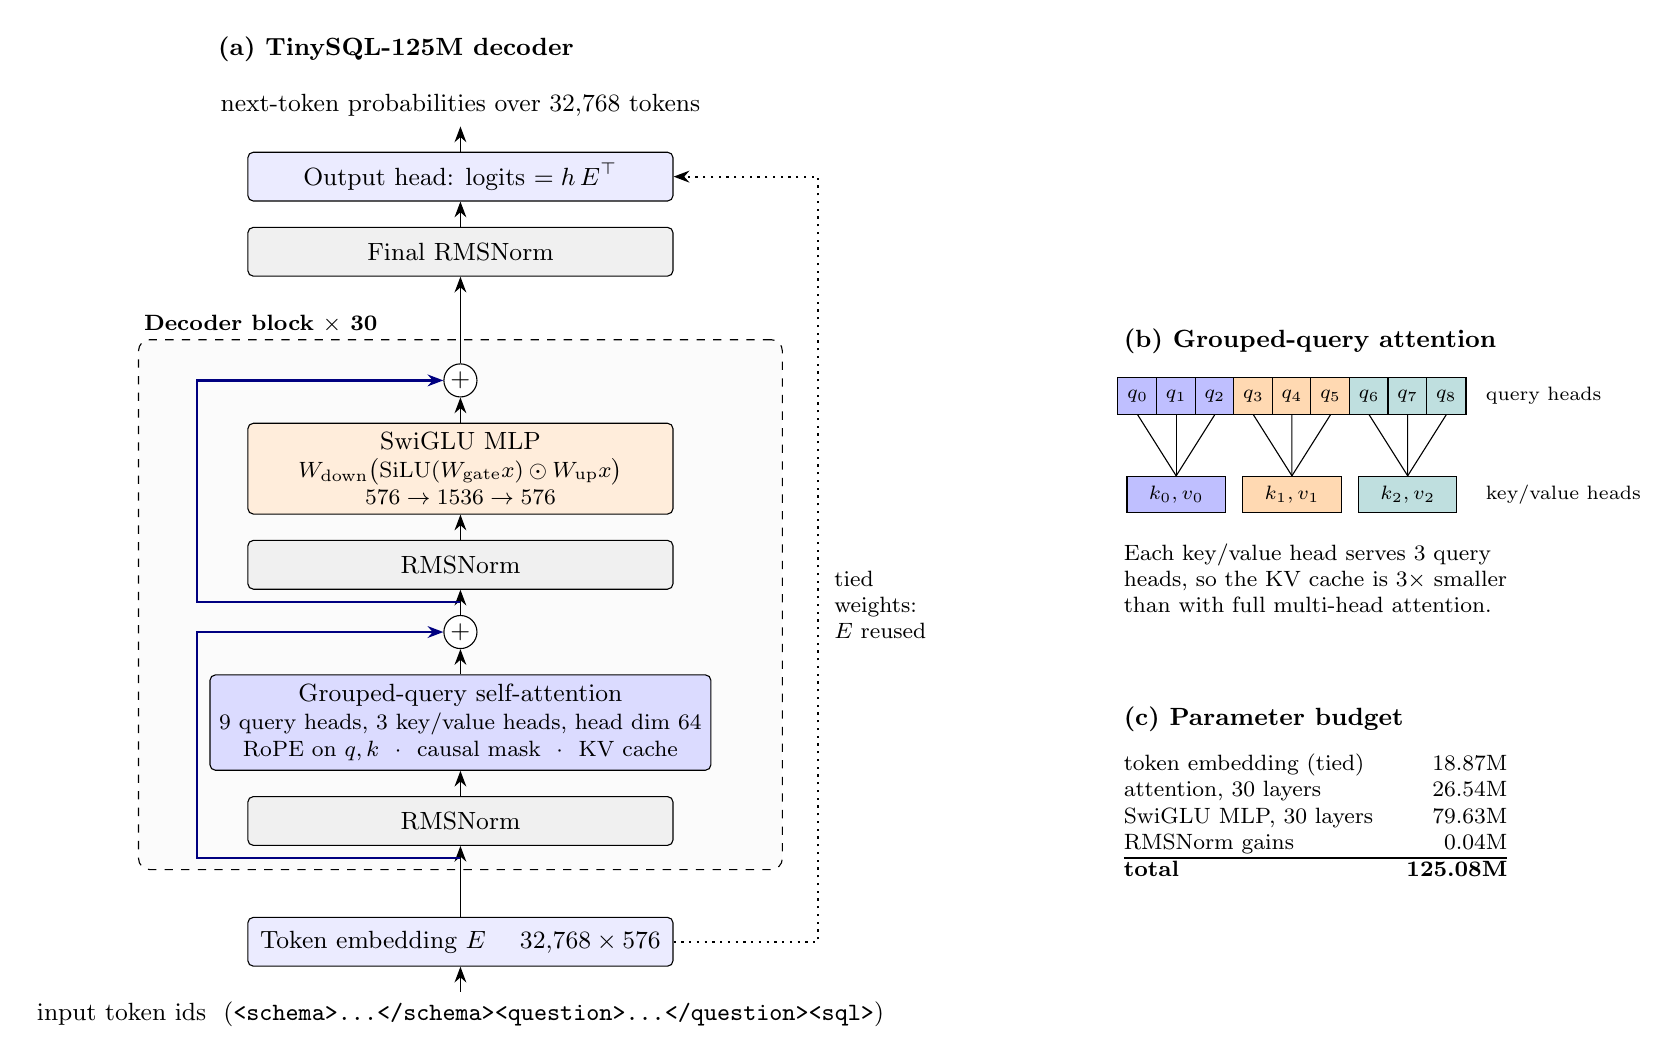
\begin{tikzpicture}[
  font=\small,
  >={Stealth[length=2mm]},
  box/.style={draw, rounded corners=2pt, minimum width=5.4cm, minimum height=0.62cm, align=center, fill=#1},
  box/.default=white,
  op/.style={draw, circle, inner sep=0pt, minimum size=4.2mm, fill=white},
  io/.style={align=center},
  panel/.style={font=\bfseries\small, anchor=west},
  node distance=3.2mm,
]
% ---------------- (a) decoder stack, bottom to top ----------------
\node[io] (ids) {input token ids \ (\texttt{<schema>\dots</schema><question>\dots</question><sql>})};
\node[box=blue!8, above=of ids] (emb) {Token embedding $E$ \quad $32{,}768 \times 576$};

\node[box=gray!12, above=9mm of emb] (n1) {RMSNorm};
\node[box=blue!14, above=of n1, minimum height=1.05cm] (att) {Grouped-query self-attention\\[-1pt]\footnotesize 9 query heads, 3 key/value heads, head dim 64\\[-1pt]\footnotesize RoPE on $q,k$ \ $\cdot$ \ causal mask \ $\cdot$ \ KV cache};
\node[op, above=of att] (add1) {$+$};
\node[box=gray!12, above=of add1] (n2) {RMSNorm};
\node[box=orange!14, above=of n2, minimum height=1.05cm] (mlp) {SwiGLU MLP\\[-1pt]\footnotesize $W_{\text{down}}\big(\mathrm{SiLU}(W_{\text{gate}}x)\odot W_{\text{up}}x\big)$\\[-1pt]\footnotesize $576 \rightarrow 1536 \rightarrow 576$};
\node[op, above=of mlp] (add2) {$+$};

\node[box=gray!12, above=11mm of add2] (nf) {Final RMSNorm};
\node[box=blue!8, above=of nf] (head) {Output head: logits $= h\,E^{\top}$};
\node[io, above=of head] (out) {next-token probabilities over 32,768 tokens};

% block frame with its own heading
\begin{scope}[on background layer]
  \node[draw, dashed, rounded corners=4pt, fit=(n1)(att)(add1)(n2)(mlp)(add2), inner xsep=9mm, inner ysep=3mm, fill=gray!3] (blk) {};
\end{scope}
\node[anchor=south west, font=\footnotesize\bfseries, inner sep=2pt] at (blk.north west) {Decoder block $\times$ 30};

% main path
\draw[->] (ids) -- (emb);
\draw[->] (emb) -- (n1);
\draw[->] (n1) -- (att);
\draw[->] (att) -- (add1);
\draw[->] (add1) -- (n2);
\draw[->] (n2) -- (mlp);
\draw[->] (mlp) -- (add2);
\draw[->] (add2) -- (nf);
\draw[->] (nf) -- (head);
\draw[->] (head) -- (out);

% residual connections (blue)
\coordinate (r1) at ($(n1.south)+(0,-0.15)$);
\draw[->, thick, blue!50!black] (r1) -- ++(-3.35,0) |- (add1.west);
\coordinate (r2) at ($(add1.north)!0.5!(n2.south)$);
\draw[->, thick, blue!50!black] (r2) -- ++(-3.35,0) |- (add2.west);

% weight tying
\coordinate (tie) at ($(blk.east |- emb.east)+(0.45,0)$);
\draw[dotted, thick, ->] (emb.east) -- (tie) |- (head.east);
\node[font=\footnotesize, align=left, anchor=west] at ($(tie |- blk.center)+(0.08,0)$) {tied\\weights:\\$E$ reused};

\node[panel] at ($(out.north)+(-3.2,0.45)$) {(a) TinySQL-125M decoder};

% ---------------- (b) GQA panel ----------------
\begin{scope}[xshift=8.6cm, yshift=6.6cm]
  \node[panel] at (-0.3,1.95) {(b) Grouped-query attention};
  \foreach \i in {0,...,8} {
    \pgfmathsetmacro{\g}{int(\i/3)}
    \ifcase\g \def\c{blue!25}\or \def\c{orange!30}\or \def\c{teal!25}\fi
    \node[draw, minimum size=4.6mm, fill=\c, font=\scriptsize] (q\i) at (\i*0.49,1.25) {$q_{\i}$};
  }
  \node[font=\scriptsize, anchor=west] at (4.3,1.25) {query heads};
  \foreach \j in {0,1,2} {
    \ifcase\j \def\c{blue!25}\or \def\c{orange!30}\or \def\c{teal!25}\fi
    \node[draw, minimum width=1.25cm, minimum height=4.6mm, fill=\c, font=\scriptsize] (kv\j) at (\j*1.47+0.49,0) {$k_{\j}, v_{\j}$};
    \pgfmathtruncatemacro{\a}{3*\j}\pgfmathtruncatemacro{\b}{3*\j+1}\pgfmathtruncatemacro{\cc}{3*\j+2}
    \draw (q\a.south) -- (kv\j.north); \draw (q\b.south) -- (kv\j.north); \draw (q\cc.south) -- (kv\j.north);
  }
  \node[font=\scriptsize, anchor=west] at (4.3,0) {key/value heads};
  \node[font=\footnotesize, align=left, anchor=north west] at (-0.3,-0.5) {Each key/value head serves 3 query\\heads, so the KV cache is $3\times$ smaller\\than with full multi-head attention.};
\end{scope}

% ---------------- (c) parameter budget ----------------
\begin{scope}[xshift=8.6cm, yshift=3.2cm]
  \node[panel] at (-0.3,0.55) {(c) Parameter budget};
  \node[font=\footnotesize, anchor=north west] at (-0.3,0.25) {%
    \begin{tabular}{@{}lr@{}}
    token embedding (tied) & 18.87M\\
    attention, 30 layers & 26.54M\\
    SwiGLU MLP, 30 layers & 79.63M\\
    RMSNorm gains & 0.04M\\
    \hline
    \textbf{total} & \textbf{125.08M}
    \end{tabular}};
\end{scope}
\end{tikzpicture}
}
\caption{\textbf{Model architecture.} (a)~The Llama-style pre-norm decoder: 30 identical blocks between a token embedding and an output head that reuses the embedding matrix (tied weights); blue lines are residual connections. (b)~Grouped-query attention: each of the 3 key/value heads serves 3 of the 9 query heads. (c)~Parameter budget by component.}
\label{fig:arch}
\end{figure}

Table~\ref{tab:arch} and Figure~\ref{fig:arch} show the model architecture. Weights start from $\mathcal{N}(0, 0.02)$, with residual output projections scaled by $1/\sqrt{2L}$. The loss is a custom autograd function that keeps only the logits and one log-sum-exp per token. This lets us fit micro-batches of up to 8$\times$2048 tokens through a 32,768-way-output layer on a 24\,GB GPU.

\subsection{Pretraining data}

\begin{table}[t]
\centering
\small
\begin{tabular}{lrrr}
\toprule
Source & Documents & Tokens & Share of shards \\
\midrule
FineWeb-Edu~\cite{penedo2024fineweb} & 3,589,789 & 3.84B & 71.0\% \\
The Stack, SQL subset~\cite{kocetkov2022stack} & 612,761 & 1.42B & 26.3\% \\
Stack Exchange (dba, datascience) & 122,659 & 0.12B & 2.2\% \\
Gretel synthetic text-to-SQL~\cite{gretel2024synthetic} ($\times$3) & 99,164 & 0.025B & 0.5\% \\
\midrule
Total & & 5.41B & \\
\bottomrule
\end{tabular}
\caption{\textbf{Pretraining corpus:} shards after cleaning, deduplication and decontamination. The mix actually trained on is set by sampling weights (Section~\ref{sec:pretrain}).}
\label{tab:data}
\end{table}

Table~\ref{tab:data} lists the sources. The pipeline applies per-source quality filters (for example, \texttt{INSERT}-heavy SQL dumps are truncated to keep the schema and drop bulk data rows), exact deduplication across all sources, and MinHash-LSH near-duplicate removal~\cite{broder1997minhash} for SQL files. From the SQL files, the 70\% with the most query features (\texttt{SELECT}, \texttt{JOIN}, \texttt{GROUP BY}, aggregates, and so on) are kept.

\paragraph{Decontamination.} Every pretraining document was scanned for WikiSQL dev and test questions: any shared 13-gram for questions of 13 or more words, or the whole question for questions of 8 to 12 words. No document matched in 4.7M scanned. Because a scanner that finds nothing proves little by itself, we ran a positive control through the same code: 200 dev/test questions planted into 1,000 real documents were all flagged, with no false positives. Questions shorter than 8 words (14\%) are too generic to scan and gold SQL strings were not scanned; both are limitations.

\subsection{Pretraining}
\label{sec:pretrain}

We train with our own AdamW~\cite{loshchilov2019adamw} ($\beta = (0.9, 0.95)$, weight decay 0.1 on weight matrices only), gradient clipping at 1.0, bf16 autocast and \texttt{torch.compile}. The peak learning rate of $1.2\times10^{-3}$ comes from a sweep on a 25M-parameter proxy (optimum near $1.4$--$1.5\times10^{-3}$, lowered for the larger model and longer run), with 200 warmup steps and cosine decay to 10\%. Each step is 524,288 tokens; the run is 8,600 steps, i.e.\ 4.51B tokens or about $3.4\times10^{18}$ FLOPs, roughly 1.8$\times$ the compute-optimal token count for this size~\cite{hoffmann2022chinchilla}. Data is mixed in two phases (Figure~\ref{fig:mix}): 82/15/2.5/0.5\% (web/SQL/Stack Exchange/Gretel) for the first 85\% of steps, then 54/36/8/2\% while the learning rate decays, so the specialised data is concentrated where the learning rate is low.

\begin{figure}[!htbp]
\centering
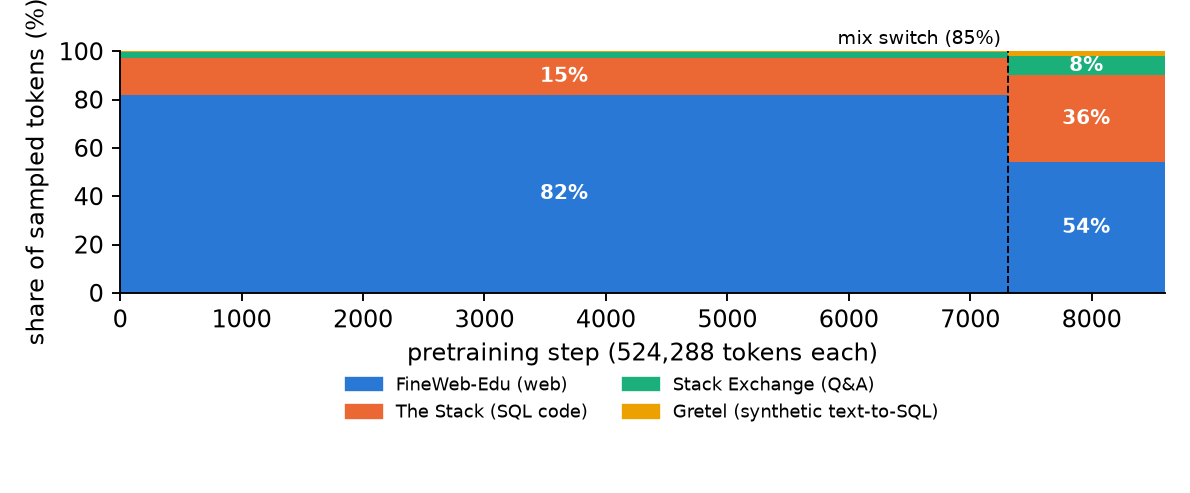
\includegraphics[width=0.85\linewidth]{data_mix.png}
\caption{\textbf{Pretraining data mix:} share of sampled tokens per source over the run. Sources are sampled at training time from fixed shards, so the mix can change without re-tokenising.}
\label{fig:mix}
\end{figure}

The run took about 46 hours on one NVIDIA L4 at 27k tokens/s (about 17\% model FLOPs utilisation), with zero skipped steps. Final validation loss is 2.94 nats/token on FineWeb-Edu and 0.96 on SQL code; every source improved at every checkpoint (Figure~\ref{fig:loss}).

\begin{figure}[!htbp]
\centering
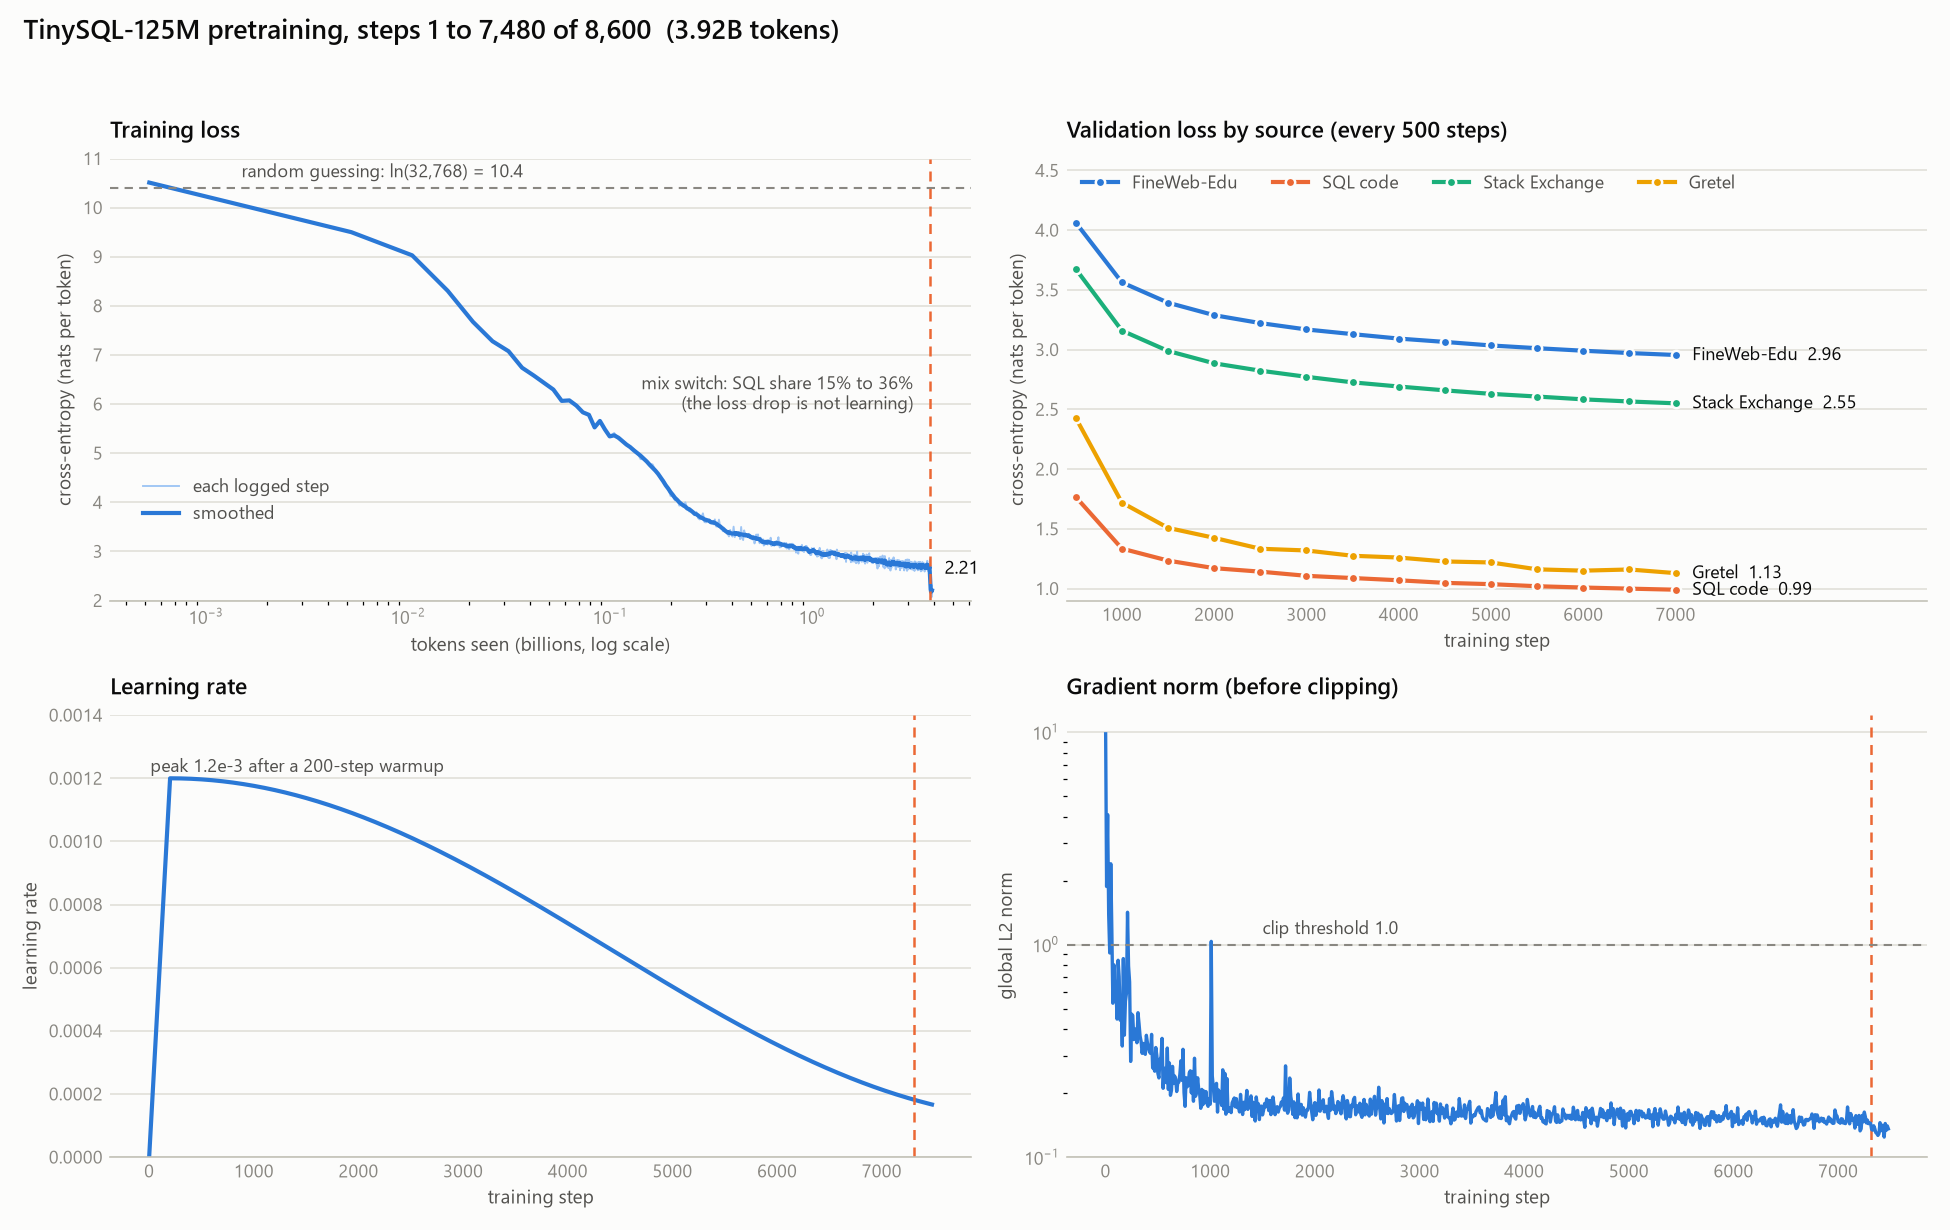
\includegraphics[width=0.8\linewidth]{loss_curves.png}
\caption{\textbf{Pretraining curves:} training loss, validation loss per source, learning rate and gradient norm over the 8,600 steps. The drop in training loss at the mix switch (step 7,310) reflects the easier SQL-heavy mix and was predicted from the per-source losses beforehand.}
\label{fig:loss}
\end{figure}

\subsection{Fine-tuning and decoding}

Each WikiSQL example turns into a pair: a prompt with the table schema as a \texttt{CREATE TABLE} statement and the question, and a completion with the SQL. The loss is calculated from the completion alone.
\begin{lstlisting}
<schema>CREATE TABLE t ("Player" TEXT, "No." TEXT, "Nationality" TEXT, "Position" TEXT, "Years in Toronto" TEXT, "School/Club Team" TEXT);</schema>
<question>What position does the player who played for butler cc (ks) play?</question>
<sql>SELECT "Position" FROM t WHERE "School/Club Team" = 'Butler CC (KS)';</sql>
\end{lstlisting}
Fine-tuning uses batch 32, 100 warmup steps, cosine decay, no weight decay and 3 epochs (5,283 steps, about 30 minutes on the L4). After each epoch, execution accuracy is measured on the first 1,000 dev questions and the best epoch is kept.

\paragraph{Constrained decoding.} Two facts about WikiSQL motivate it. 95\% of our model's invalid greedy outputs reference a column that does not exist, and 100\% of gold condition values (11,545 of 11,545 on dev) occur verbatim, ignoring case, in the question. We therefore define two levels. \emph{Schema} is a byte-level grammar for the WikiSQL query shape that only admits the table's real column names. \emph{Schema + values} additionally requires every condition value to be a substring of the question (Unicode-aware, valid UTF-8). At each step, candidate tokens are checked best-first and the first that keeps the output a valid prefix is taken, which is equivalent to masking every invalid token and taking the argmax (Figure~\ref{fig:constrained}). The same decoder runs on the baselines through a byte-level adapter for their tokenizers.

\begin{figure}[!htbp]
\centering
\resizebox{0.95\linewidth}{!}{% Constrained decoding, one step at a time: candidates are checked best-first against the grammar.
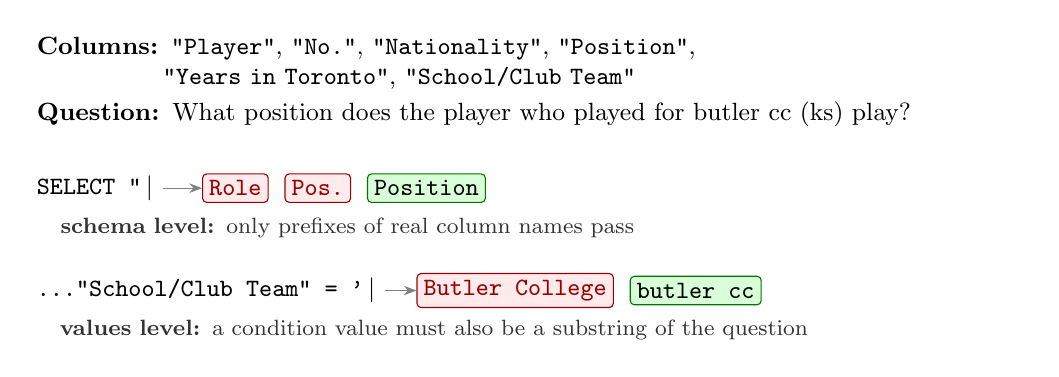
\begin{tikzpicture}[
  font=\small,
  >={Stealth[length=1.6mm]},
  tok/.style={draw, rounded corners=1.5pt, inner sep=2.4pt, font=\ttfamily\small},
  ok/.style={tok, fill=green!15, draw=green!45!black},
  bad/.style={tok, fill=red!8, draw=red!60!black, text=red!60!black},
  note/.style={anchor=west, align=left, font=\footnotesize, text width=4.6cm},
]
\node[align=left, anchor=west, text width=12.5cm] (ctx) at (0,0) {%
  \textbf{Columns:} \texttt{"Player"}, \texttt{"No."}, \texttt{"Nationality"}, \texttt{"Position"},\\
  \hspace*{1.6cm}\texttt{"Years in Toronto"}, \texttt{"School/Club Team"}\\[2pt]
  \textbf{Question:} What position does the player who played for butler cc (ks) play?};

% step 1: column
\node[anchor=west] (p1) at (0,-1.35) {\texttt{SELECT "}\,\(\vert\)};
\node[bad, right=5mm of p1] (c11) {Role};
\node[bad, right=2mm of c11] (c12) {Pos.};
\node[ok, right=2mm of c12] (c13) {Position};
\node[note, text width=12cm, gray!40!black] at (0.3,-1.85) {\textbf{schema level:} only prefixes of real column names pass};
\draw[->, gray] (p1) -- (c11);

% step 2: value
\node[anchor=west] (p2) at (0,-2.65) {\texttt{\dots"School/Club Team" = '}\,\(\vert\)};
\node[bad, right=4mm of p2] (c21) {Butler College};
\node[ok, right=2mm of c21] (c22) {butler cc};
\node[note, text width=12cm, gray!40!black] at (0.3,-3.15) {\textbf{values level:} a condition value must also be a substring of the question};
\draw[->, gray] (p2) -- (c21);
\end{tikzpicture}
}
\caption{\textbf{Constrained decoding} on a WikiSQL dev question (candidate tokens are illustrative). Candidates are tried left to right in model-score order: red ones would leave the grammar and are skipped, green is the first valid one. Checking is lazy, so usually only a few candidates are tested; the result equals masking every invalid token and taking the argmax.}
\label{fig:constrained}
\end{figure}

\section{Experimental setup}
\label{sec:setup}

\paragraph{Baselines.} We fine-tuned models from GPT-2 124M~\cite{radford2019gpt2}, Pythia-160M~\cite{biderman2023pythia}, SmolLM2-135M and SmolLM2-360M~\cite{benallal2025smollm2} using the same prompt text, loss masking, batch size, AdamW optimiser, schedule, epochs and epoch selection. The baselines accumulate gradients over token-weighted micro-batches, which a test shows gives the same gradient as the full batch to $10^{-6}$. Our architecture was also fine-tuned from random weights with the same recipe.

\paragraph{Protocol.}
\begin{enumerate}
  \item \textbf{Learning rate}, per model, from $\{5\times10^{-5}, 10^{-4}, 2\times10^{-4}\}$ (control: $\{10^{-4}, 10^{-3}\}$), chosen on the first 1,000 dev questions (Figure~\ref{fig:lr}; Table~\ref{tab:lr} in the appendix).
  \item \textbf{Seeds:} three for TinySQL and both SmolLM2 models; one for GPT-2, Pythia and the control.
  \item \textbf{Test set, once:} the dev-phase weights had been deleted after scoring, so every system was fine-tuned again with its dev-chosen configuration and scored on test exactly once. No decision was made after seeing a test number.
\end{enumerate}

\begin{figure}[!htbp]
\centering
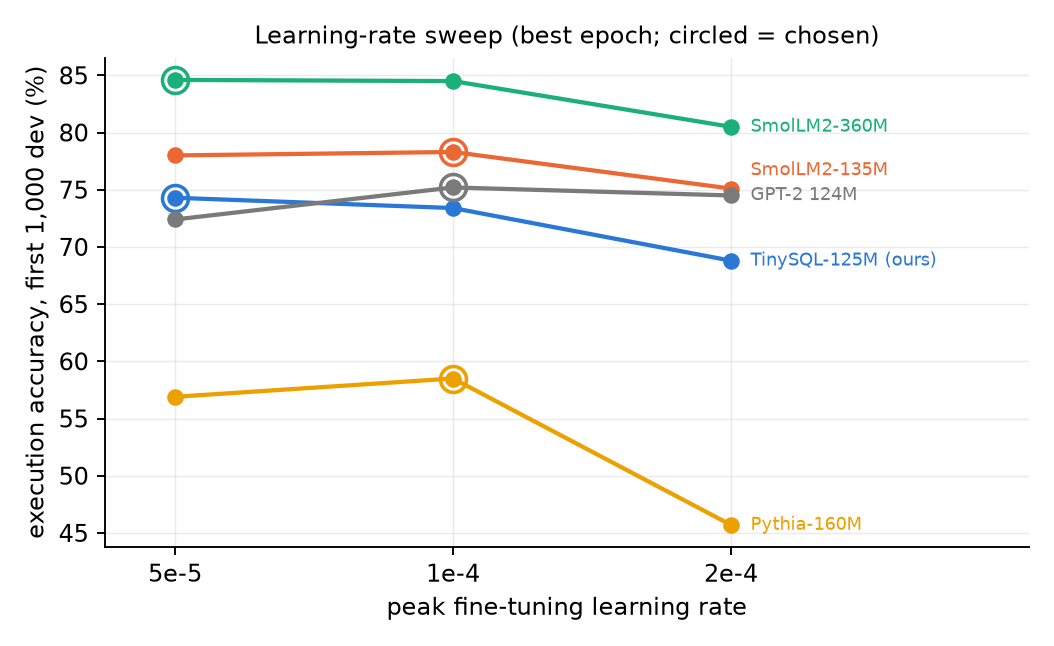
\includegraphics[width=0.7\linewidth]{lr_sweep.png}
\caption{\textbf{Learning-rate sweep} for fine-tuning, seed 0. Every model gets its own best learning rate; $2\times10^{-4}$ is too high for all of them.}
\label{fig:lr}
\end{figure}

\paragraph{Metrics.} Our main measure is how accurately the predicted queries match the gold queries when both are run against the table in a sandboxed read-only SQLite connection. We also use Salesforce's official WikiSQL evaluator, which gives scores for both execution and logical-form accuracy. When we feed the gold queries as predictions, it scores exactly 100\% on the dev and test sets. Its execution accuracy matches ours within 0.11 points across all runs of the four main systems.

\paragraph{Statistics.} For each system we report the mean and standard deviation over seeds and a 95\% percentile-bootstrap confidence interval~\cite{efron1993bootstrap} over questions, using 10,000 resamples of the seed-averaged per-question accuracy. Comparisons between systems pair their seed-0 predictions question by question, using a paired bootstrap~\cite{koehn2004significance} and the exact McNemar test~\cite{mcnemar1947} on the questions where exactly one system is correct, following~\cite{dror2018hitchhiker}.

\section{Results}
\label{sec:results}

\subsection{Main results}

\begin{table}[t]
\centering
\small
\begin{tabular}{lrcccc}
\toprule
Model & \shortstack[r]{Pretraining\\tokens} & Seeds & Greedy & + Schema & \shortstack{+ Schema\\+ values} \\
\midrule
\textbf{TinySQL-125M (ours)} & \textbf{4.5B} & 3 & \textbf{\pmstd{77.95}{0.18}} & 79.06 & \textbf{\pmstd{80.39}{0.20}} \\
GPT-2 124M & unknown & 1 & 78.93 & 80.07 & 82.36 \\
Pythia-160M & 300B & 1 & 60.78 & 63.98 & 67.63 \\
SmolLM2-135M & 2T & 3 & \pmstd{82.57}{0.37} & 83.16 & \pmstd{85.22}{0.21} \\
SmolLM2-360M & 4T & 3 & \pmstd{87.03}{0.19} & 87.42 & \pmstd{88.01}{0.12} \\
\midrule
Ours, no pretraining & 0 & 1 & 37.39 & -- & 48.33 \\
\bottomrule
\end{tabular}
\caption{\textbf{Main results:} WikiSQL \textbf{test} execution accuracy (\%, 15,878 questions). Mean $\pm$ std over seeds; schema-only uses seed 0. 95\% bootstrap CIs are $\pm$0.5 to 0.8 points (Table~\ref{tab:official} and the repository). Dev results (Table~\ref{tab:dev}) agree closely.}
\label{tab:main}
\end{table}

\begin{table}[t]
\centering
\small
\begin{tabular}{lrrr}
\toprule
Comparison (test, greedy) & Difference [95\% CI] & Discordant & $p$ (McNemar) \\
\midrule
SmolLM2-360M $-$ ours & +9.20 [+8.6, +9.8] & 1940 / 480 & $<10^{-200}$ \\
SmolLM2-135M $-$ ours & +4.16 [+3.6, +4.8] & 1532 / 871 & $8\times10^{-42}$ \\
GPT-2 $-$ ours & +0.91 [+0.3, +1.5] & 1287 / 1142 & 0.0035 \\
Pythia-160M $-$ ours & $-$17.23 [$-$18.0, $-$16.5] & 647 / 3383 & $<10^{-300}$ \\
Ours $-$ no pretraining & +40.62 [+39.8, +41.4] & 6704 / 254 & $<10^{-300}$ \\
\bottomrule
\end{tabular}
\caption{\textbf{Paired significance tests} on test (seed 0). ``Discordant'' counts questions only the first system answers correctly, then questions only the second does.}
\label{tab:paired}
\end{table}

Table~\ref{tab:main} gives test accuracy and Table~\ref{tab:paired} the paired comparisons. Figure~\ref{fig:tokens} places each model by its pretraining tokens.

\begin{enumerate}
  \item \textbf{Pretraining is most of the result.} The same network fine-tuned from random weights reaches 37.4\%. Pretraining on 4.5B tokens adds 40.6 points, and constrained decoding cannot substitute for it (48.3\% even with both constraints).
  \item \textbf{About one point behind GPT-2.} GPT-2 is ahead by 0.9 points at greedy ($p = 0.004$) and 2.0 points with both constraints. On dev the greedy gap was 0.5 points and not significant ($p = 0.26$), so we report the test result: GPT-2 is slightly better.
  \item \textbf{Far ahead of Pythia-160M,} by 17 points at greedy, despite Pythia's 67$\times$ larger pretraining budget. Pythia invents column names far more often (8.5\% of test questions produce invalid SQL, vs 2.0\% for ours). Our ablation (Section~\ref{sec:ablations}) suggests that the SQL-heavy mix explains only a small part of this gap, so we do not claim a cause.
  \item \textbf{Scale still wins at equal size:} SmolLM2-135M, with about 440$\times$ our pretraining tokens, is 4.6 points ahead (mean over seeds), and SmolLM2-360M is 9.1 points ahead.
  \item \textbf{Results are stable.} Seed standard deviations are 0.1--0.4 points, far smaller than every gap between models. Our dev-to-test drop is 0.7 points, similar to the baselines' 0.4--0.5 (Pythia, whose fine-tuning is unstable, drops 5 points).
\end{enumerate}

\begin{figure}[!htbp]
\centering
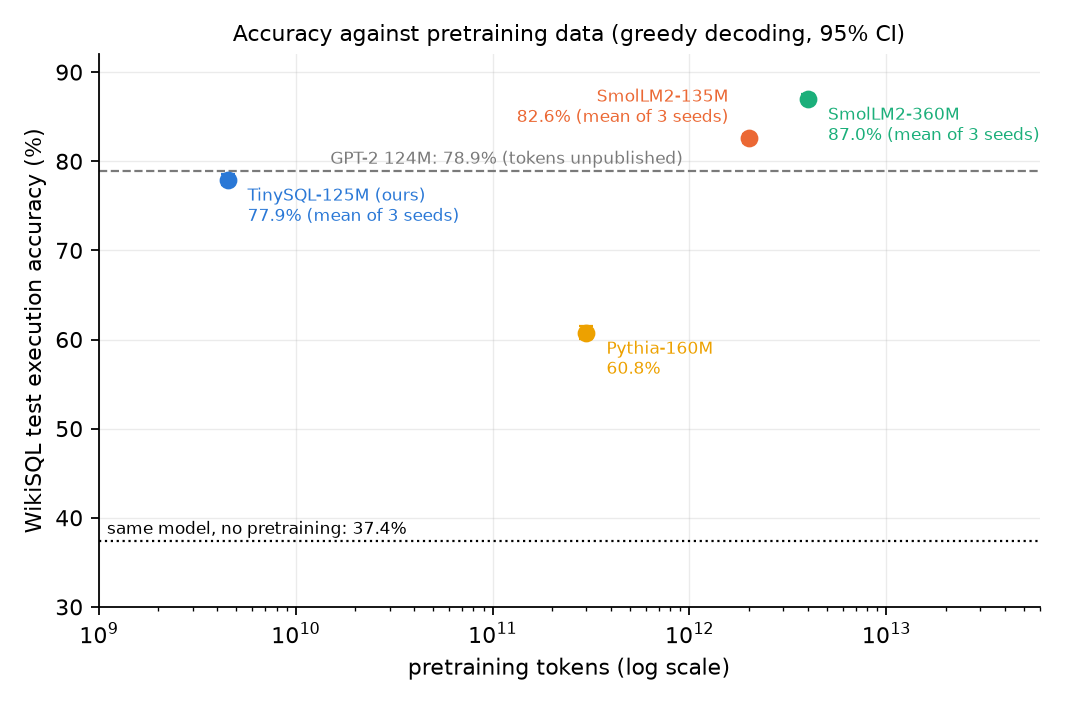
\includegraphics[width=0.8\linewidth]{accuracy_vs_tokens_test.png}
\caption{\textbf{Accuracy vs.\ pretraining data:} test execution accuracy (greedy, 95\% CI) against pretraining tokens. GPT-2's token count is not published, so it is drawn as a reference line, as is our no-pretraining control.}
\label{fig:tokens}
\end{figure}

\subsection{Constrained decoding}

\begin{table}[t]
\centering
\small
\begin{tabular}{lccc}
\toprule
Model & + Schema & + Schema + values & Fixed / broken (schema + values) \\
\midrule
TinySQL-125M (ours) & +1.05 & +2.42 & 385 / \textbf{0} \\
GPT-2 124M & +1.14 & +3.43 & 659 / 114 \\
Pythia-160M & +3.19 & +6.85 & 1495 / 407 \\
SmolLM2-135M & +0.98 & +2.81 & 483 / 37 \\
SmolLM2-360M & +0.21 & +0.94 & 189 / 40 \\
No pretraining & -- & +10.94 & 1755 / 18 \\
\bottomrule
\end{tabular}
\caption{\textbf{Gains from constrained decoding} over greedy decoding with the same weights (test, seed 0, points; all $p < 0.005$). ``Fixed'' and ``broken'' count questions that change from wrong to right and from right to wrong.}
\label{tab:constrained}
\end{table}

Constraints raise validity to 100\% for every model and help weaker models more (Table~\ref{tab:constrained}, Figure~\ref{fig:gains}).

\begin{figure}[!htbp]
\centering
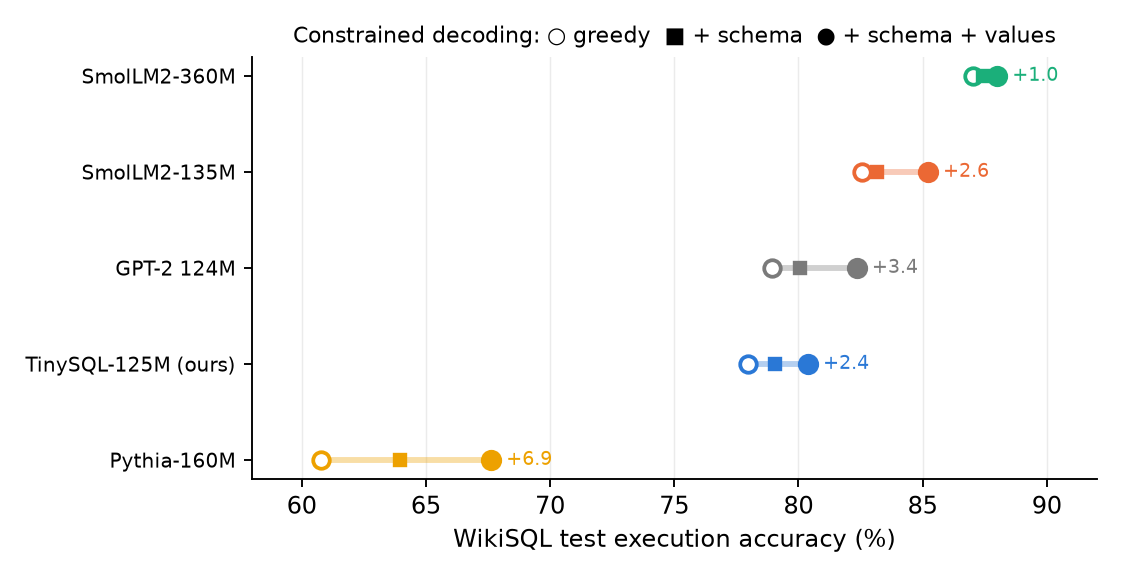
\includegraphics[width=0.8\linewidth]{decoding_gains.png}
\caption{\textbf{Gains from constrained decoding:} test accuracy with greedy decoding (open circle), the schema constraint (square) and schema + values (filled circle); mean over seeds where available. The gain shrinks as the model gets stronger.}
\label{fig:gains}
\end{figure}

The value constraint is worth more than the schema constraint for every model: copying filter values exactly is where small models slip most. For our model, constrained decoding \emph{never} turned a correct answer into a wrong one in any paired comparison we ran (0 broken on test at both levels; 0 on dev). For every baseline it sometimes does, plausibly because their tokenizers can be forced into token splits they rarely produce; we did not verify this.

\subsection{Ablations}
\label{sec:ablations}

\begin{table}[t]
\centering
\small
\begin{tabular}{lcccc}
\toprule
Variant (one change from base) & Params & Dev accuracy & $\Delta$ & $p$ \\
\midrule
\textbf{Base} (RoPE, GQA 6/2, tied, mixed data) & 25.2M & \textbf{55.82} [54.8, 56.9] & & \\
Learned absolute positions instead of RoPE & 25.6M & 47.35 & $-$8.48 & $7\times10^{-89}$ \\
Untied input/output embeddings & 37.8M & 50.83 & $-$5.00 & $6\times10^{-32}$ \\
Full multi-head attention & 26.7M & 55.08 & $-$0.75 & 0.055 \\
Web text only (no SQL, code or Q\&A) & 25.2M & 54.89 & $-$0.94 & 0.021 \\
\bottomrule
\end{tabular}
\caption{\textbf{Ablations} on a 25M-parameter proxy (8 layers, $d = 384$, context 1024), each pretrained on 150M tokens and fine-tuned with the same recipe. Greedy dev execution accuracy, one seed each; $p$ from McNemar against the base.}
\label{tab:ablations}
\end{table}

\begin{figure}[!htbp]
\centering
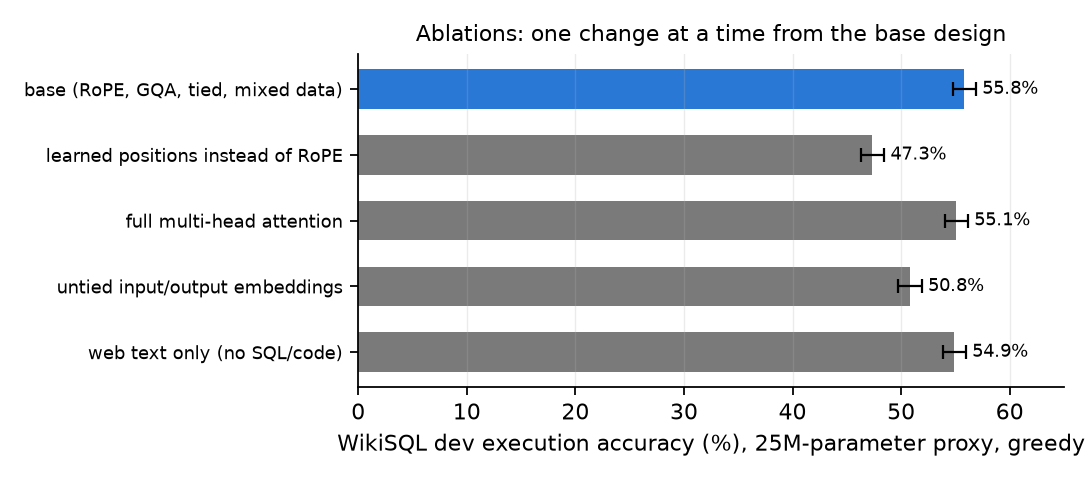
\includegraphics[width=0.8\linewidth]{ablations.png}
\caption{\textbf{Ablations} on the 25M proxy: one design change at a time from the base model (dev, greedy, 95\% CI).}
\label{fig:ablations}
\end{figure}

Table~\ref{tab:ablations} and Figure~\ref{fig:ablations} vary one design choice at a time on a small proxy model. Rotary embeddings matter most: without them, accuracy drops 8.5 points and pretraining loss is clearly worse (4.51 vs 4.09 nats on web text). Tying embeddings helps by 5 points even though the untied model has 50\% more parameters. Grouped-query attention costs nothing measurable while shrinking the KV cache 3$\times$. Most surprisingly, removing all SQL, code and Q\&A data from pretraining costs only 0.9 points after fine-tuning, even though the web-only model's loss on SQL code is far higher (4.40 vs 1.81 nats). Fine-tuning on 56k WikiSQL examples appears to recover most of what the SQL data teaches. These are single-seed results at 150M tokens, so we treat them as indicative.

\subsection{Failure analysis}
\label{sec:failures}

\begin{figure}[!htbp]
\centering
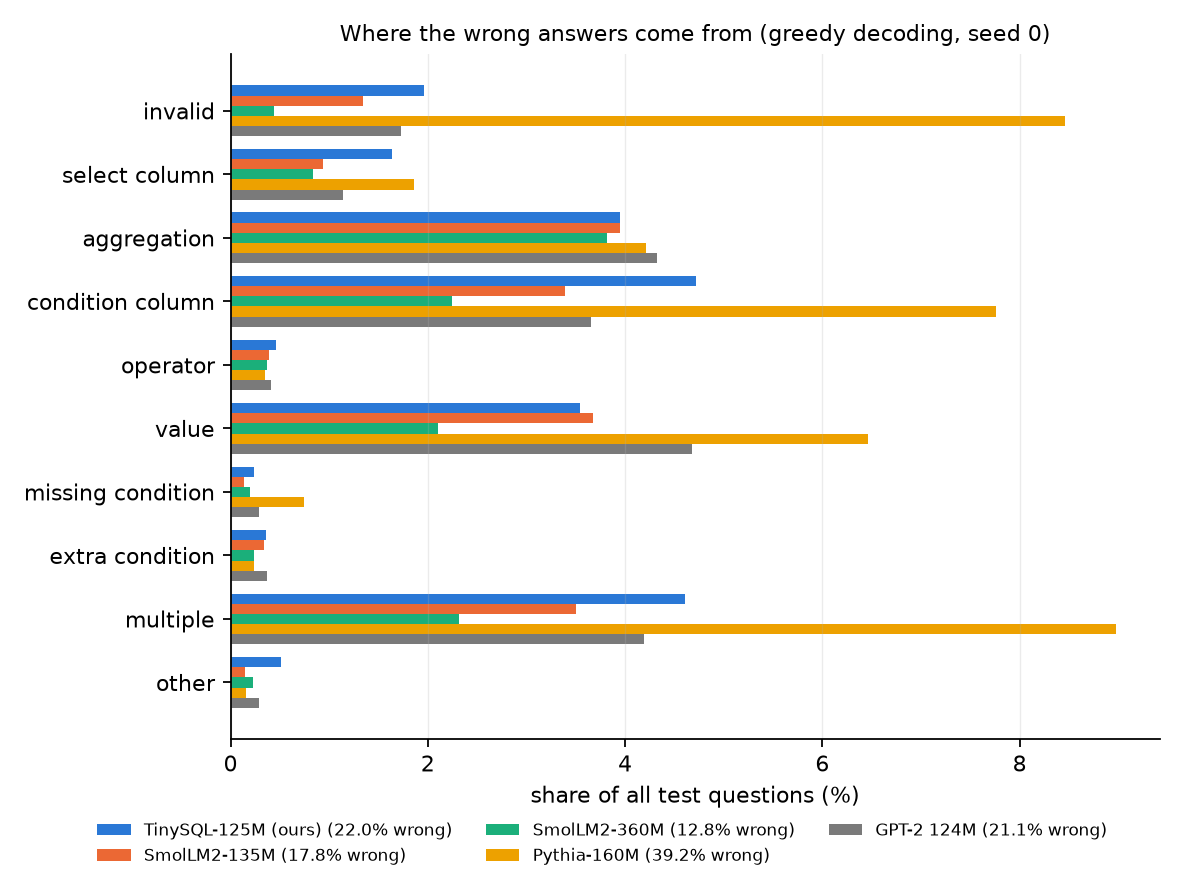
\includegraphics[width=0.85\linewidth]{failure_categories_test.png}
\caption{\textbf{Failure categories:} where wrong answers come from (test, greedy, seed 0). Each wrong prediction is parsed into WikiSQL's structured form and assigned exactly one category.}
\label{fig:failures}
\end{figure}

Each wrong prediction is parsed back into WikiSQL's structure (selected column, aggregation, conditions) and compared with gold, giving exactly one category (Figure~\ref{fig:failures}). Compared with stronger models, our model loses most on condition columns, values and multi-part errors, the skills that depend on reading the table and the question. Aggregation errors are different: they stay at 3.8--4.3\% of test questions for every pretrained model, although overall accuracy spans 26 points.

\paragraph{Query complexity.} Accuracy falls when the gold query needs more conditions (Figure~\ref{fig:conds}). On the 10,832 single-condition test questions, our model and GPT-2 are level (80.3\% and 80.2\%, seed 0). The gap widens with two conditions (73.5\% versus 76.2\% on 3,879 questions), which matches the multi-part errors in Figure~\ref{fig:failures}. Pythia drops fastest, from 64.5\% to 35.8\% at four conditions.

\begin{figure}[!htbp]
\centering
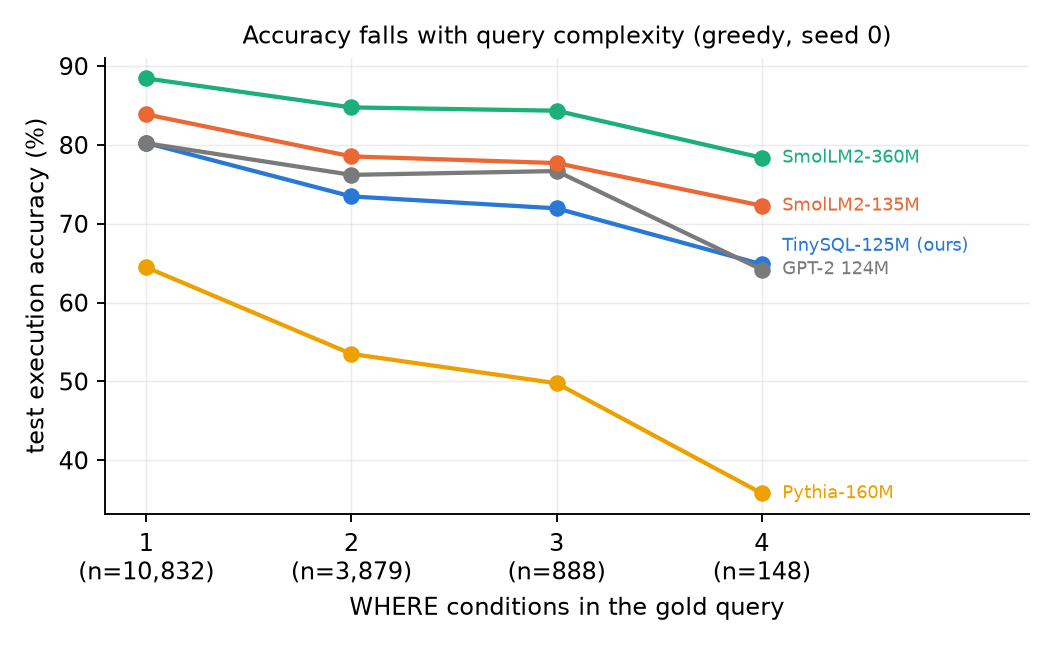
\includegraphics[width=0.7\linewidth]{accuracy_by_conditions.png}
\caption{\textbf{Accuracy by query complexity:} test accuracy by the number of WHERE conditions in the gold query (greedy, seed 0). The 131 questions without conditions are omitted.}
\label{fig:conds}
\end{figure}

\paragraph{Aggregation label audit.} To find out why, we hand-checked 50 randomly sampled dev questions where our model was wrong \emph{only} in the aggregation. In 31 (62\%; 95\% Wilson CI~\cite{wilson1927} 48--74\%) the gold aggregation is not supported by the question. For example, ``How many people were in the crowd when Essendon was the home team?'' is labelled \texttt{COUNT(Crowd)} rather than the crowd figure, and ``For record 25-24, what is the sum of attendance?'' is labelled \texttt{COUNT}. A further 12 (24\%) are ambiguous, and only 7 (14\%) are clear model errors. Extrapolated, roughly 2 points of dev accuracy are lost to aggregation labels for every model, which is consistent with earlier reports of annotation errors in WikiSQL~\cite{hwang2019sqlova,pihulski2025llmsql}. The audit had a single annotator (the author), not blinded; all 50 judgements are released for re-checking.

\section{Limitations}

\begin{itemize}
  \item \textbf{One benchmark, one query shape.} WikiSQL queries are single-table with no joins, grouping or nesting. We do not evaluate on harder benchmarks such as Spider~\cite{yu2018spider}.
  \item \textbf{Uncontrolled baseline pretraining.} The baselines differ in pretraining data, tokenizers and architecture, not just in token count, so Figure~\ref{fig:tokens} shows association, not a scaling law.
  \item \textbf{One pretraining run.} Seeds vary fine-tuning only. GPT-2, Pythia, the control and all ablations have a single fine-tuning seed.
  \item \textbf{Noisy selection.} Learning rates and epochs are selected on 1,000 dev questions, whose 95\% CI is about $\pm$2.8 points, wider than the differences between adjacent learning rates.
  \item \textbf{Reproducibility on GPU.} Fine-tuning is not bit-reproducible on GPU even with fixed seeds. Pythia's re-fine-tune for test, for example, differs from its dev run.
  \item \textbf{Decontamination} covers dev/test questions of 8 or more words, not short questions or SQL strings. The audit is single-annotator.
\end{itemize}

\section{Conclusion}

A single developer can build every component of a text-to-SQL language model, pretrain it on 4.5B tokens in two days on one GPU, and land within about one point of GPT-2 on WikiSQL while outperforming a model pretrained on 67$\times$ more data. Constrained decoding is a cheap and safe addition at this scale. Getting the last points still requires much more pretraining, and on WikiSQL a measurable share of the remaining errors are in the labels rather than in the models.

\section*{Reproducibility}

The code, configurations, prediction-level results, statistics and figures are in \url{https://github.com/aditya0929/tinysql}. Every run, every number and every bug found along the way are recorded in \texttt{PROJECT\_LOG.md}. Pretraining took about 46 L4 GPU-hours, and the benchmark (fine-tuning, evaluation and ablations) took about 45, both on NVIDIA L4 GPUs.

\bibliographystyle{plainnat}
\bibliography{refs}

\appendix
\section{Additional results}

\begin{table}[h]
\centering
\small
\begin{tabular}{lcccc}
\toprule
Model & $5\times10^{-5}$ & $10^{-4}$ & $2\times10^{-4}$ & Chosen \\
\midrule
TinySQL-125M & 74.3 & 73.4 & 68.8 & $5\times10^{-5}$ \\
SmolLM2-135M & 78.0 & 78.3 & 75.1 & $10^{-4}$ \\
SmolLM2-360M & 84.6 & 84.5 & 80.5 & $5\times10^{-5}$ \\
GPT-2 124M & 72.4 & 75.2 & 74.5 & $10^{-4}$ \\
Pythia-160M & 56.9 & 58.5 & 45.7 & $10^{-4}$ \\
\bottomrule
\end{tabular}
\caption{\textbf{Learning-rate sweep (numbers):} execution accuracy on the first 1,000 dev questions, best epoch, seed 0. Control: 28.6 ($10^{-4}$) vs 11.5 ($10^{-3}$).}
\label{tab:lr}
\end{table}

\begin{table}[h]
\centering
\small
\begin{tabular}{lccc}
\toprule
Model & Greedy & + Schema & + Schema + values \\
\midrule
TinySQL-125M (ours) & \pmstd{78.63}{0.26} & 79.68$^*$ & \pmstd{80.96}{0.21} \\
GPT-2 124M & 79.41 & 80.60 & 82.79 \\
Pythia-160M & 65.94 & 68.38 & 72.15 \\
SmolLM2-135M & \pmstd{82.97}{0.22} & 83.46$^*$ & \pmstd{85.45}{0.22} \\
SmolLM2-360M & \pmstd{87.40}{0.20} & 87.55$^*$ & \pmstd{88.41}{0.10} \\
No pretraining & 37.70 & -- & 48.22 \\
\bottomrule
\end{tabular}
\caption{\textbf{Dev results:} WikiSQL \textbf{dev} execution accuracy (\%, 8,421 questions). $^*$Single run at learning rate $10^{-4}$.}
\label{tab:dev}
\end{table}

\begin{table}[h]
\centering
\small
\begin{tabular}{lcccc}
\toprule
& \multicolumn{2}{c}{Execution} & \multicolumn{2}{c}{Logical form} \\
\cmidrule(lr){2-3}\cmidrule(lr){4-5}
Model & Greedy & + Schema + values & Greedy & + Schema + values \\
\midrule
TinySQL-125M (ours) & \pmstd{78.03}{0.19} & \pmstd{80.50}{0.20} & \pmstd{72.28}{0.09} & \pmstd{74.48}{0.07} \\
GPT-2 124M & 78.94 & 82.35 & 73.25 & 76.41 \\
Pythia-160M & 61.02 & 68.04 & 55.10 & 61.17 \\
SmolLM2-135M & \pmstd{82.61}{0.35} & \pmstd{85.27}{0.19} & \pmstd{77.42}{0.39} & \pmstd{79.91}{0.25} \\
SmolLM2-360M & \pmstd{87.00}{0.17} & \pmstd{87.99}{0.10} & \pmstd{81.71}{0.17} & \pmstd{82.66}{0.10} \\
No pretraining & 37.64 & 48.46 & 31.60 & 40.76 \\
\bottomrule
\end{tabular}
\caption{\textbf{Official evaluator:} WikiSQL \textbf{test} scores from Salesforce's evaluate.py (\%). 95\% bootstrap CIs (our executor) for the greedy rows: ours [77.4, 78.5], GPT-2 [78.3, 79.6], Pythia [60.0, 61.5], SmolLM2-135M [82.0, 83.1], SmolLM2-360M [86.6, 87.5], no pretraining [36.7, 38.1].}
\label{tab:official}
\end{table}

\end{document}
